\chapter{Dataset and Experimental Methodology}
\label{ch:data}

\section{Equity Universe and Data Acquisition}
The experimental stock universe comprises $N = 10$ prominent large-cap equities actively traded on the National Stock Exchange of India (NSE), spanning diverse economic sectors:
\begin{enumerate}
    \setlength{\itemsep}{1pt}
    \item \textbf{RELIANCE.NS} (Energy and Petrochemicals / Conglomerate)
    \item \textbf{TCS.NS} (Information Technology Services)
    \item \textbf{HDFCBANK.NS} (Private Commercial Banking)
    \item \textbf{ICICIBANK.NS} (Private Commercial Banking)
    \item \textbf{ITC.NS} (Consumer Goods and Diversified Conglomerate)
    \item \textbf{HINDUNILVR.NS} (Fast-Moving Consumer Goods)
    \item \textbf{LT.NS} (Engineering and Infrastructure Construction)
    \item \textbf{SUNPHARMA.NS} (Pharmaceuticals and Healthcare)
    \item \textbf{MARUTI.NS} (Automotive Manufacturing)
    \item \textbf{BHARTIARTL.NS} (Telecommunications and Digital Services)
\end{enumerate}
In addition to these ten equities, the portfolio includes an explicit cash asset (Asset 11), providing the agent with the operational flexibility to hold liquidity and de-risk during volatile market phases.

Daily price and volume records were acquired from Yahoo Finance via the \texttt{yfinance} API spanning 1 January 2009 to 31 December 2025. Data acquisition utilized \texttt{auto\_adjust=True}: price series (Open, High, Low, and Close) are backward-adjusted for both stock splits and cash dividends, whereas trading volume is adjusted for splits. Data from 2009--2010 serves as an initial burn-in buffer to initialize 200-day moving averages, ensuring that all technical indicators are fully settled by 1 January 2011. The common trading calendar comprises 3,699 active trading days.

\section{Feature Engineering and Market Indicators}
For each asset $i \in \{1, \dots, N\}$ on trading day $t$, a compact feature vector $\mathbf{f}_{i,t} \in \mathbb{R}^{13}$ is computed using causal market and technical price transformations. To ensure cross-asset comparability, features are normalized by prevailing prices or rolling averages:

\begin{enumerate}
    \setlength{\itemsep}{2pt}
    \item \textbf{Daily Log Return ($f_{1,i,t}$):} $r_{i,t}^{\text{log}} = \ln\left( C_{i,t} / C_{i,t-1} \right)$.
    \item \textbf{Close-to-Open Relative Return ($f_{2,i,t}$):} $o_{i,t}^{\text{rel}} = C_{i,t} / O_{i,t} - 1$.
    \item \textbf{High-to-Low Relative Spread ($f_{3,i,t}$):} $hl_{i,t}^{\text{rel}} = H_{i,t} / L_{i,t} - 1$.
    \item \textbf{Normalized Relative Volume ($f_{4,i,t}$):} $v_{i,t}^{\text{rel}} = \ln\left( V_{i,t} / \text{SMA}_{20}(V_{i,t}) \right)$.
    \item \textbf{50-day EMA Relative Deviation ($f_{5,i,t}$):} $ema_{50,i,t}^{\text{rel}} = C_{i,t} / \text{EMA}_{50}(C_{i,t}) - 1$, with smoothing multiplier $\alpha_n = \frac{2}{n+1}$.
    \item \textbf{200-day EMA Relative Deviation ($f_{6,i,t}$):} $ema_{200,i,t}^{\text{rel}} = C_{i,t} / \text{EMA}_{200}(C_{i,t}) - 1$.
    \item \textbf{Relative Strength Index ($f_{7,i,t}$):} Wilder's 14-period RSI centered around zero:
    \begin{equation}
    \text{RS}_{i,t} = \frac{\bar{U}_{i,t}}{\bar{D}_{i,t} + 10^{-8}}, \quad \text{RSI}_{i,t} = 100 - \frac{100}{1 + \text{RS}_{i,t}}, \quad f_{7,i,t} = \frac{\text{RSI}_{i,t}}{100} - 0.5.
    \end{equation}
    \item \textbf{Moving Average Convergence Divergence ($f_{8,i,t}$):} Normalized trend divergence:
    \begin{equation}
    \text{MACD}_{i,t} = \frac{\text{EMA}_{12}(C_{i,t}) - \text{EMA}_{26}(C_{i,t})}{C_{i,t}}.
    \end{equation}
    \item \textbf{MACD Signal Line ($f_{9,i,t}$):} $\text{Signal}_{i,t} = \text{EMA}_9(\text{MACD}_{i,t}) / C_{i,t}$.
    \item \textbf{Average True Range ($f_{10,i,t}$):} Normalized price volatility:
    \begin{equation}
    \text{ATR}_{i,t}^{\text{rel}} = \frac{\text{SMA}_{14}(\text{TR}_{i,t})}{C_{i,t}}, \quad \text{where } \text{TR}_t = \max(H_t - L_t, |H_t - C_{t-1}|, |L_t - C_{t-1}|).
    \end{equation}
    \item \textbf{Bollinger Band \%B ($f_{11,i,t}$):} Position relative to 2-standard-deviation envelopes:
    \begin{equation}
    \%B_{i,t} = \frac{C_{i,t} - \text{LB}_{i,t}}{\text{UB}_{i,t} - \text{LB}_{i,t} + 10^{-8}}.
    \end{equation}
    \item \textbf{Bollinger Bandwidth ($f_{12,i,t}$):} Volatility width: $\text{BW}_{i,t} = (\text{UB}_{i,t} - \text{LB}_{i,t}) / \text{MB}_{i,t}$.
    \item \textbf{Average Directional Index ($f_{13,i,t}$):} Wilder's 14-period normalized trend: $\text{ADX}_{i,t}^{\text{norm}} = \text{ADX}_{14,i,t} / 100$.
\end{enumerate}

\section{State Representation and Temporal Sequences}
The instantaneous observation vector concatenates the 13 features across all $N = 10$ equities ($130$ market features) with the current portfolio weight vector $\mathbf{w}_t^{\text{cur}} \in \mathbb{R}^{N+1}$ (10 equities plus cash, 11 weights):
\begin{align}
\mathbf{x}_t &= \text{concat}\left(\mathbf{f}_{1,t}, \dots, \mathbf{f}_{N,t}\right) \in \mathbb{R}^{130}, \\
\mathbf{s}_t &= \left[ \mathbf{x}_t^\top, \; (\mathbf{w}_t^{\text{cur}})^\top \right]^\top \in \mathbb{R}^{141}.
\end{align}
The total daily state dimension is $D_{\text{state}} = 141$. For models using recurrent memory (M2--M4), a sliding historical window of $W = 30$ trading days is maintained:
\begin{equation}
\mathbf{F}_t = \left[ \mathbf{s}_{t-W+1}, \dots, \mathbf{s}_t \right]^\top \in \mathbb{R}^{30 \times 141}.
\end{equation}
Feature standardization is fitted strictly on the training partition of each fold using mean $\boldsymbol{\mu}_{\text{train}}$ and standard deviation $\boldsymbol{\sigma}_{\text{train}}$, with standardized values clipped to $[-5.0, 5.0]$. All features use causal backward operators, preventing look-ahead leakage.

\section{Walk-Forward Evaluation Protocol}
Following \citet{liu2024dynamic}, models are trained and tested using an 8-year rolling-origin walk-forward protocol across four folds. Each fold consists of 6 years of training data, 1 year of validation data, and 2 years of held-out out-of-sample test data, advancing by 2 years per fold (Table~\ref{tab:folds_overview} and Figure~\ref{fig:walk_forward}).

\begin{table}[htbp]
\centering
\small
\setlength{\tabcolsep}{4pt}
\caption{Chronological specification of the four walk-forward folds.}
\label{tab:folds_overview}
\begin{tabularx}{\textwidth}{c>{\centering\arraybackslash}X>{\centering\arraybackslash}X>{\centering\arraybackslash}Xcc}
\toprule
\textbf{Fold} & \textbf{Training Period (6y)} & \textbf{Validation Period (1y)} & \textbf{Test Period (2y)} & \textbf{Training Trading Days} & \textbf{Test Trading Days} \\
\midrule
1 & 2011-01-01 to 2016-12-31 & 2017-01-01 to 2017-12-31 & 2018-01-01 to 2019-12-31 & 1,478 & 489 \\
2 & 2013-01-01 to 2018-12-31 & 2019-01-01 to 2019-12-31 & 2020-01-01 to 2021-12-31 & 1,475 & 496 \\
3 & 2015-01-01 to 2020-12-31 & 2021-01-01 to 2021-12-31 & 2022-01-01 to 2023-12-31 & 1,476 & 495 \\
4 & 2017-01-01 to 2022-12-31 & 2023-01-01 to 2023-12-31 & 2024-01-01 to 2025-12-31 & 1,479 & 494 \\
\bottomrule
\end{tabularx}
\end{table}

The test periods are non-overlapping and span 2018 through 2025. It is important to distinguish the number of historical trading days in the dataset splits ($\approx 1,478$ training days and $\approx 490$ test days) from the reinforcement learning training budget, which is fixed at 300,000 environment interaction steps across all models.

\begin{figure}[htbp]
\centering
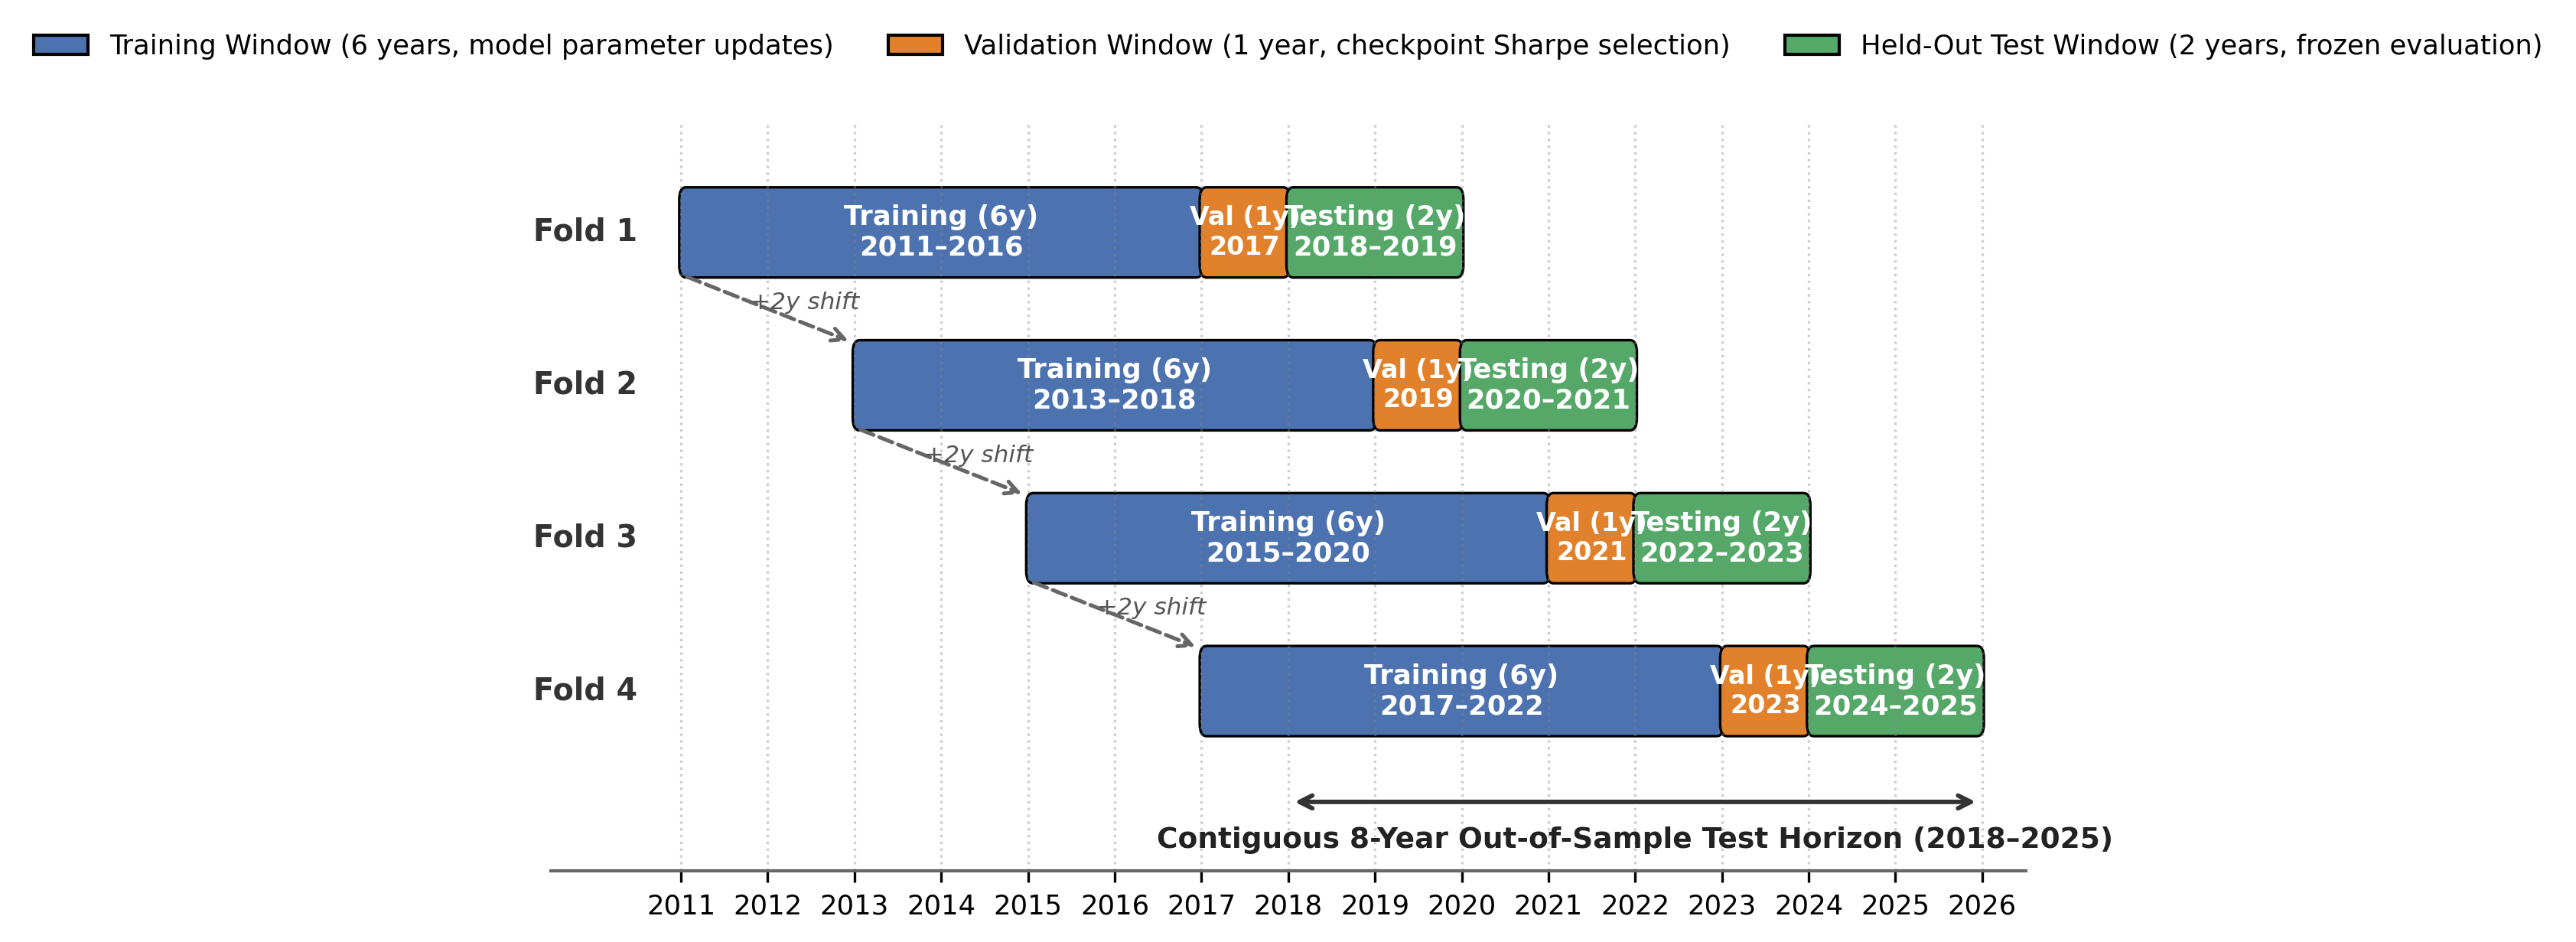
\includegraphics[width=0.92\textwidth]{figures/walk_forward_schematic.png}
\caption{Chronological four-fold rolling walk-forward evaluation protocol with 6-year training, 1-year validation, and 2-year testing windows, advancing by 2 years per fold (adapted from Liu et al. (2024), Figure 5).}
\label{fig:walk_forward}
\end{figure}

To assess statistical variability, each configuration is trained across three fixed random seeds ($S \in \{0, 1, 2\}$). During training, validation Sharpe ratio is evaluated periodically every 25,000 environment steps, and the checkpoint achieving the highest validation Sharpe ratio is saved. At the conclusion of 300,000 steps, this best-validation checkpoint is restored and evaluated once on the out-of-sample test window. 

\textit{Methodological Disclosure:} We note that earlier exploratory runs of Model M1 were conducted on Fold 1 test data during preliminary system debugging. We distinguish those preliminary debugging iterations from the final reported runs; test-set feedback was not used to adjust hyperparameters or select architectures.
